\documentclass{article}

\usepackage{amsmath}
\usepackage{amssymb}
\usepackage{algorithm}
\usepackage[noend]{algpseudocode}		% for algorithms in pseudo code. Usage: \begin{algorithmic}
\usepackage{tikz}
\usepackage{subcaption}

\newcommand{\vecl}{\overrightarrow} % long vector for multiple characters
\newcommand{\ang}[1]{\measuredangle\left( #1 \right)}
\newcommand{\len}[1]{\left\lVert #1 \right\rVert}
\newcommand{\inta}[1]{\operatorname{int}\left( #1 \right)} % interior angle
\newcommand{\exta}[1]{\operatorname{ext}\left( #1 \right)} % exterior angle

\title{Determining the Convexity of any Polygon}
\author{Abraham Murciano}

\begin{document}
\maketitle

\section{Abstract}

This paper presents and proves the correctness of an algorithm which determines if a sequence of points in three-dimensional space forms a convex polygon or not. We will discuss simple concave polygons as well as complex (self intersecting) polygons. As an added bonus, we will be able to detect and reject any input whose vertices do not lie on a common plane.

\section{Definitions}

\begin{description}
	\item[Angle between vectors]
		The angle between two three-dimensional vectors \(\vec{u}\) and \(\vec{v}\), which we shall denote henceforth as \(\ang{\vec{u}, \vec{v}}\), is defined as follows.
		\begin{equation*}
			\ang{\vec{u}, \vec{v}} = \arccos \left( \frac{\vec{u} \cdot \vec{v}} {\len{\vec{u}} \cdot \len{\vec{v}}} \right)
		\end{equation*}
		It is important to note that \(\ang{\vec{u}, \vec{v}}\) is always between 0 and \(\pi\) radians. For any two vectors there are two angles between them, and the function \(\measuredangle\) always gives us the smaller of the two.

	\item[Polygon]
		A polygon is a \emph{plane} figure that is described by a finite number of straight line segments connected to form a closed circuit. The enclosed plane region, as well as the bounding circuit, is what we shall call a polygon.

	\item[Simple polygon]
		A simple polygon is a polygon whose bounding line segments do not intersect with each other.

	\item[Interior angle]
		For a simple polygon, an angle between two adjacent line segments is called an interior angle (or internal angle) if a point within the angle is in the interior of the polygon. A simple polygon has exactly one internal angle per vertex.

		We shall denote the interior angle at vertex \(Q\) as \(\inta{Q}\).

	\item[Exterior angle]
		If \(P\), \(Q\), and \(R\) are three consecutive points of a sequence of points (such that \(Q\) is in between \(P\) and \(R\)), the exterior angle of the sequence at the point \(Q\) is \(\exta{Q} = \ang{\vecl{PQ}, \vecl{QR}}\).

		Note, since the range of the function \(\measuredangle\) is \([0, \pi]\), by `exterior angle' we refer always (unless otherwise noted) to a positive angle.

	\item[Convex polygon]
		A polygon is convex if it is simple and all its interior angles are less than \(\pi\) radians.

	\item[Concave polygon]
		A polygon is concave if it is simple and not convex.

	\item[Complex polygon]
		A polygon is complex if it is not simple, i.e. if its edges intersect with each other. There is debate whether or not complex polygons are considered polygons, but for the purposes of this paper we shall refer to them as polygons.
\end{description}

\begin{figure}[htbp]
	\centering
	\begin{subfigure}{0.25\textwidth}
		\centering
		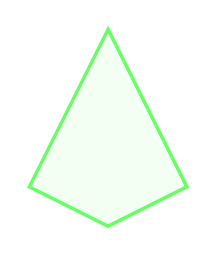
\begin{tikzpicture}
			\filldraw[color=green!60, fill=green!5, very thick] (0, 0) -- (1, -0.5) -- (2, 0) -- (1, 2) -- cycle;
		\end{tikzpicture}
		\caption{Convex}
	\end{subfigure}%
	\begin{subfigure}{0.25\textwidth}
		\centering
		
\begin{tikzpicture}
			\filldraw[color=orange!60, fill=orange!5, very thick] (0, 0) -- (1, 0.5) -- (2, 0) -- (1, 2.5) -- cycle;
		\end{tikzpicture}
		\caption{Concave}
	\end{subfigure}%
	\begin{subfigure}{0.25\textwidth}
		\centering
		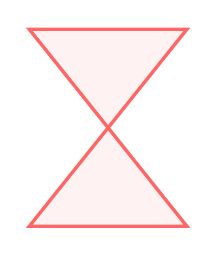
\begin{tikzpicture}
			\filldraw[color=red!60, fill=red!5, very thick] (0, 0) -- (2, 2.5) -- (0, 2.5) -- (2, 0) -- cycle;
		\end{tikzpicture}
		\caption{Complex}
	\end{subfigure}%
	\caption{Examples of different types of polygons.}
	\label{}
\end{figure}

\section{The Algorithm}

We will begin by explaining how the algorithm works, then presenting the algorithm at the end of this section.

\subsection{Input}

The algorithm accepts a sequence of points in three-dimensional space. The points, if they share a common plane, represent a polygon formed by constructing an edge between all adjacent vertices in the sequence and an additional edge between the first and last vertices.

\subsection{Output}

The algorithm returns True if the input forms a convex polygon, and False otherwise.

Some examples of when the input does not form a convex polygon are
\begin{itemize}
	\item if the points form a concave polygon,
	\item if the points form a complex polygon, and
	\item if the points do not share a common plane, and thus do not form a polygon at all.
\end{itemize}

\subsection{Processing}

The algorithm boils down to a single check. A sequence of vertices forms a simple convex polygon if and only if the sum of the exterior angles is equal to \(2\pi\). Formally, the algorithm checks if the following equation holds true, where \(V\) is the input sequence of vertices.

\begin{equation*}
	\sum_{v \in V} \exta{v} = 2\pi
\end{equation*}

\subsection{Pseudo Code}

The function \textsc{IsConvex} takes as input a sequence of points \(V\) and returns whether or not the points form a convex polygon.

\begin{algorithm}[htbp]
	\begin{algorithmic}
		\Function{IsConvex}{$V$}
		\If{\(|V| < 3\)}
		\Return False
		\EndIf
		\State \(s := 0\) \Comment{The sum of the exterior angles.}
		\For{\(i\) from 0 to \(|V| - 1\)}
		\State \(P := V_{i-1 \mod |V|}\) \Comment{The previous point.}
		\State \(Q := V_{i}\) \Comment{The current point.}
		\State \(R := V_{i+1 \mod |V|}\) \Comment{The next point.}
		\State \(s := s + \ang{\vecl{PQ}, \vecl{QR}}\) \Comment{Add the exterior angle of \(Q\).}
		\EndFor
		\State\Return \(s = 2\pi\)
		\EndFunction
	\end{algorithmic}
\end{algorithm}

\section{Proof of Correctness}

\subsection{Claim}

A sequence of vertices \(V\) forms a simple convex polygon if and only if the sum of the exterior angles is equal to \(2\pi\).

In order to prove our claim, we must prove all of the following cases.
\begin{enumerate}
	\item If a polygon is convex then the sum of its exterior angles is equal to \(2\pi\).
	\item If a polygon is concave then the sum of its exterior angles is greater than \(2\pi\).
	\item If a polygon is complex then the sum of its exterior angles is greater than \(2\pi\).
	\item If all points in a sequence do not share a common plane, then the exterior angles of the points have a sum greater than \(2\pi\).
\end{enumerate}

\subsection{Proof}

\subsubsection{Convex Polygons' Exterior Angles Sum to \(2\pi\)}

Suppose a convex polygon is drawn on the ground, and we are standing on one of the edges, facing parallel to the edge with our right foot inside the polygon and our left foot outside. We shall call the direction that we are currently facing the initial direction. Then if we walk forward following the the edges of the polygon, and at each vertex we turn to face the next vertex, turning whichever way (right or left) is a smaller turn. Eventually we would reach the starting edge again.

At each of the vertices we turned toward the right an amount equal to the exterior angle. It must be the case that we always turn to the right, since every interior angle is less than \(\pi\) radians (by definition of convex), and the inside of the polygon is to our right. See figure \ref{walk-1}.

\begin{figure}[htbp]
	\centering
	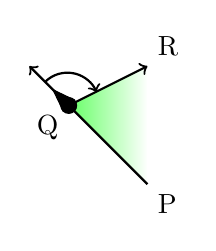
\begin{tikzpicture}
		\shadedraw[->, thick, left color=green!60, right color=white] (0, 0) node[anchor=north west] {P}
		to (-1, 1) node[anchor=north east] {Q}
		to (0, 1.5) node[anchor=south west] {R};
		\draw[->, thick] (-1, 1) to (-1.5, 1.5);
		\filldraw (-1, 1) circle (0.1);
		\filldraw (-1.2, 1.2) to (-1.07, 0.93) to (-0.93, 1.07) to cycle;
		\draw[->, thick] (-1.3, 1.3) arc (135:22.5:0.4);
	\end{tikzpicture}
	\caption{Turns at a vertex of a convex polygon are always right turns.}
	\label{walk-1}
\end{figure}

Since we always turned to our right, and we ended up facing the initial direction, and at no other edge or vertex were we facing the initial direction, it must be that in total we turned precisely one rotation, that is, \(2\pi\).

Thus the total amount we turned (\(2\pi\)) must be equal to the sum of the amounts we turned at each vertex (\(\sum_{v \in V}\exta{v}\)).

\subsubsection{A Concave Polygon's Exterior Angles' Sum exceeds \(2\pi\)}

Suppose once again that a polygon is drawn on the ground, but this time let it be concave. Again, suppose we are starting on any edge facing parallel to it with our right foot inside the polygon. This is our initial direction. Suppose we again walk the edges in the same way as we walked the convex polygon.

At some point, we will reach a vertex whose interior angle is greater than \(\pi\) radians (by definition of concave). When this occurs, we will find that the next vertex is on our left hand side, and we will have to turn in that direction (see figure \ref{walk-2}). Since eventually we must reach the starting point and be facing the initial direction, we must at some point turn enough to the right to correct for our leftward deviation. This means that for every interior angle greater than \(\pi\) radians, we will add both the deviation and the correction to the complete turn of \(2\pi\) which we must eventually make.

\begin{figure}
	\centering
	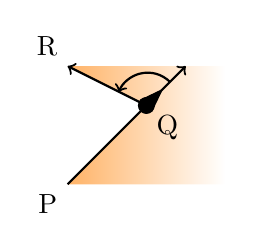
\begin{tikzpicture}
		\shade[left color=orange!60, right color=white] (2, 0) to (0, 0) to (1, 1) to (0, 1.5) to (2, 1.5) to cycle;
		\draw[->, thick] (0, 0) node[anchor=north east] {P}
		to (1, 1) node[anchor=north west] {Q}
		to (0, 1.5) node[anchor=south east] {R};
		\draw[->, thick] (1, 1) to (1.5, 1.5);
		\filldraw (1, 1) circle (0.1);
		\filldraw (1.2, 1.2) to (1.07, 0.93) to (0.93, 1.07) to cycle;
		\draw[->, thick] (1.3, 1.3) arc (45:157.5:0.4);
	\end{tikzpicture}
	\caption{A turn at an vertex \(Q\) of a concave polygon where \(\inta{Q} > \pi\), must be a left turn.}
	\label{walk-2}
\end{figure}%

The deviation at each of these vertices is \(\exta{v}\), and the correction at some future turn must match it. Let \(V' \subset V\) be the set of vertices whose interior angles are greater than \(\pi\). Formally,
\begin{equation}
	V' = \{ v \in V : \inta{v} > \pi \}.
	\label{v-prime}
\end{equation}
Therefore we have the following.
\begin{equation}
	\sum_{v \in V} \exta{v} = 2\pi + 2\sum_{v \in V'} \exta{v}
	\label{ext-concave}
\end{equation}
And since exterior angles are always positive (see definition above), and in the case of every vertex in \(V'\) not equal to zero (otherwise the interior angle would be precisely \(\pi\) contradicting equation \ref{v-prime}), equation \ref{ext-concave} must be strictly greater than \(2\pi\).

\subsubsection{A Complex polygon's Exterior Angles' Sum Exceeds \(2\pi\)}

Suppose for a third time that a polygon is drawn on the ground. This time let the polygon have self intersections and thus be complex. If we were to walk the edges like we did before, we would once again end facing the initial direction.

Reminder; a turn is made when we have concluded the traversal of a single edge, and are standing on a vertex. If the subsequent vertex is situated on our left hand side we make a left turn, otherwise we make a right turn. Remember, a turn is never negative or greater than \(\pi\) radians.

Without loss of generality, suppose the sum of the right turns is greater than or equal to the sum of the left turns. Since we must end facing the initial direction, the sum of all the right turns minus the sum of the left turns is a non-negative multiple of \(2\pi\). Let us call this value \(T\). We can now say that for some \(n \in \mathbb{N}_0\),
\begin{equation}
	T = 2\pi n
\end{equation}

We shall now branch our analysis into three cases. The first case is when \(n = 0\), the second when \(n = 1\), and the third when \(n \geq 2\).

\paragraph{Case 1.} When \(n = 0 \Rightarrow T = 2\pi \times 0 = 0\). This means that the sum of the right turns is equal to that of the left turns.

Since we started standing on an edge, this edge touches one vertex directly in front of us and another directly behind us. As we are to traverse every vertex before reaching the starting point, we must at some point reach the vertex behind us.

In order to do this without walking backwards --- for we must always walk forward in the direction we face --- we must at some edge (let us call it \(e\)) be facing `backwards'; that is strictly more than \(\frac{\pi}{2}\) radians from the initial direction. Without loss of generality, assume the described direction can be faced with a right turn from the initial direction.

In order to reach such a direction, the sum of all the previous right turns minus the sum of all the previous left turns must exceed \(\frac{\pi}{2}\) radians (a quarter turn).

Let \(R_p\) and \(L_p\) be the sum of all the previous right and left turns respectively before reaching edge \(e\). Further, let \(R_f\) and \(L_f\) be the sum of all the future right and left turns respectively after reaching edge \(e\).

We showed at the start of this case that the sums of the right and left turns are equal.
\begin{gather}
	R_p + R_f = L_p + L_f \\
	\Rightarrow R_p - L_p = L_f - R_f \label{case-1-eq1}
\end{gather}

Then we showed that the previous right turns minus the previous left turns is greater than \(\frac{\pi}{2}\).
\begin{gather}
	R_p - L_p > \frac{\pi}{2} \label{case-1-eq2} \\
	\Rightarrow R_p > L_p + \frac{\pi}{2}
\end{gather}

From equations \ref{case-1-eq1} and \ref{case-1-eq2} we show that the reverse is true for future turns.
\begin{gather}
	L_f - R_f > \frac{\pi}{2} \\
	\Rightarrow L_f > R_f + \frac{\pi}{2}
\end{gather}

\end{document}